\chapter{Criação de Base de Dados}
\label{cap:banco}
Este capítulo tem como objetivo apresentar a Rede Social Reddit na qual seu
conteúdo foi extraído para a base de dados, os tópicos
selecionados para a análise de sentimentos, e por fim, é apresentada a
ferramenta desenvolvida para a extração dos tópicos e criação da base.
\section{Rede Social Reddit}
\label{cap:Reddit}

O \textit{website} Reddit teve seu início em 2005 como um agregador de
conteúdo e, atualmente, é o vigésimo terceiro \textit{website} mais acessado na
internet e o sétimo mais acessado nos Estados Unidos da América \cite{alexa}.
Os usuários do Reddit podem enviar \textit{links} com conteúdos externos
ao Reddit ou ainda mensagens de texto. A partir desse conteúdo, os seus
usuários podem votar para cima (\textit{upvote}) ou para baixo \textit{downvote},
influenciando na posição do conteúdo no \textit{website}. Além de votar no conteúdo, seus usuários podem enviar comentários como
forma de expressar sua opinião.

\begin{figure}[!htbp]
\centering

\includegraphics[height=300px]{imagens/reddit.png}
\caption{\textit{Website Reddit}:  As flechas demarcadas permitem efetuarmos
\textit{upvotes} ou \textit{downvotes}.}
\label{fig:reddit}
\end{figure}

O conteúdo do Reddit é distribuído em \textit{subreddits} que funcionam como
comunidades que abordam certos assuntos. Os usuários podem se inscrever nesses
\textit{subreddits}, recebendo as atualizações na sua página inicial, sendo
que dentre os \textit{subreddits}, destacam-se:


\begin{itemize}
  \item \textit{/r/AskReddit}: Esse \textit{subreddit} é utilizado para fazer
  perguntas gerais para outros usuários. Esse \textit{subreddit} possui
  aproximadamente 16.941.544 de inscritos.
  \item \textit{/r/worldnews}: Esse \textit{subreddit} possui as notícias do
  mundo. Contando, aproximadamente com 16.570.606 de inscritos.
  \item \textit{/r/IAmA}: IAmA é um estilização de 'I am a' ('Eu sou um'):
  a partir desse \textit{subreddit} os usuários podem fazer perguntas ao criador
  de um determinado tópico. Esse \textit{subreddit} possui aproximadamente
  16.990.161 de inscritos.
\end{itemize}

% Dentre esses \textit{subreddits} podemos destacar alguns dos tópicos mais
% acessados no ano de 2016:
% 
% \begin{itemize}
%   \item \textit{/r/IAmA} - \textit{We're NASA scientists \& exoplanet experts.
%   Ask us anything about today's announcement of seven Earth-size planets
%   orbiting TRAPPIST-1!} - Tópico de perguntas e respostas com cientistas da
%   NASA após a descoberta dos planetas que orbitavam a estrela TRAPPIST-1.
%   \item \textit{/r/IAmA} - \textit{I’m Bill Gates, co-chair of the Bill \&
%   Melinda Gates Foundation. Ask Me Anything.} - Tópico de perguntas e respostas com Bill Gates.
%   \item \textit{/r/worldnews} - \textit{Fidel Castro is dead at 90.} - Link para
%   anúncio da morte de Fidel Castro.
%   \item \textit{/r/AskReddit} - \textit{[Serious]South Koreans of Reddit, how
%   did they teach you about the existence of North Korea in School when you were
%   young?serious replies only} - Tópico perguntando para os usuários sul coreanos
%   como que foi ensinado para eles sobre a existência da Coreia do Norte.
% \end{itemize}

% A identificação de padrões de sentimentos expressos por determinados grupos
% dessa comunidade, se faz útil visto que a partir dessa avaliação é possível construir
% ferramentas que apoiam decisões tanto de um ponto de vista político, como por
% exemplo, entender qual é a opinião sobre um determinado assunto de um conjunto
% de eleitores, tanto quanto um ponto de vista de negócios, para entender qual a
% opinião dos consumidores de um produto, ou de seu competidor, a respeito de um
% determinado assunto.

\section{Extração de Dados}
\label{cap:Extracao}

Para a extração dos dados e criação da base foi
criado um \textit{crawler} ou robô de navegação. Esse robô foi desenvolvido na
linguagem Java e tem como objetivo a navegação automática no conteúdo do
\textit{website} Reddit, extraindo os dados e comentários referentes a um
determinado tópico. Após, os dados são armazenados em banco de dados MySQL
\cite{Widenius:2002:MRM:560480}.
Na Figura \ref{fig:crawler} tem-se a arquitetura do \textit{software}
desenvolvido.

\begin{figure}[htbp]
\centering
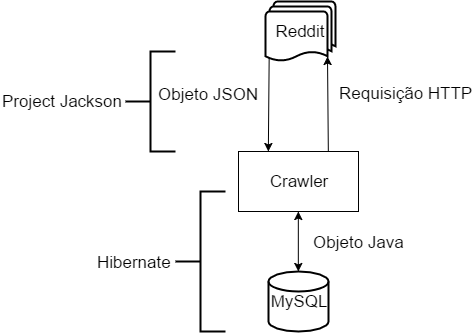
\includegraphics[height=225px]{imagens/arquitetura.png}
\caption{Arquitetura do \textit{Crawler}}
\label{fig:crawler}
\end{figure}

A partir de um \textit{link} para um tópico, o robô efetua uma busca e a
extração dos dados relacionados a esse tópico. Para tanto, foi utilizada a
\ac{API} do Reddit, onde, inicialmente envia-se uma requisição utilizando o
sufixo ``.json'' (Por exemplo:
\textit{\url{https://www.reddit.com/r/iama.json}}) e, a partir dessa requisição,
o \textit{website} retorna um objeto \ac{JSON}. Uma vez que o \ac{JSON}
retornado pelo \textit{website} possui 68 campos e que esses não se encontram
documentados, utilizou-se o \textit{website}
jsonschema2pojo\footnote{http://www.jsonschema2pojo.org/} para converter o JSON
retornado em um objeto \ac{POJO}. De fato, esse \textit{website} tem como
objetivo a conversão de um esquema \ac{JSON} em \ac{POJO}, permitindo o
\textit{download} da classe para a utilização.

Após, foi utilizado o \textit{framework} Hibernate
\cite{Iverson:2004:HJD:1044870} para a criação de banco de dados, assim como
persistência dos dados em um banco de dados MySQL, criando as tabelas
\textit{RedditPost} e \textit{RedditThread}, relacionadas respectivamente com
os comentários e o tópico em questão.
O \textit{framework} Hibernate é um \textit{framework} de mapeamento objeto-relacional que tem como objetivo representar tabelas do
banco de dados através de classes.

\section{Tópicos Selecionados}

Para análise de sentimentos e comparação dos resultados obtidos, foram
selecionados 15 tópicos. Esses tópicos são os que apresentam maior número de
comentários no último ano.

Os 15 tópicos encontram-se distribuídos em diferentes assuntos, que são: cenário
político nacional, cenário político internacional e tópicos diversos:

No que diz respeito a tópicos relacionados com ao cenário político nacional, os
tópicos escolhidos foram:
\sloppy
\begin{itemize}
  \item
  \textit{Brazil Seeks To Copy U.S. Gun Culture ``to allow embattled
  citizens the right to defend themselves from
  criminals''}: esse encontra-se disponível em 
  \url{https://www.reddit.com/r/worldnews/comments/36ny58/brazil_blogger_known_for_reporting_on_corruption/}
  e refere-se a intenção do Brasil de copiar a cultura de porte de armas dos
  Estados Unidos da América.
  \item
  \textit{Brazil descends into chaos as Olympics looms}: esse encontra-se disponível em 
  \url{https://www.reddit.com/r/worldnews/comments/4bqcc3/brazil_descends_into_chaos_as_olympics_looms/}
  e refere-se ao caos ocorrido nas Olímpiadas realizadas no Brasil.
  \item
  \textit{Plane carrying Brazil Supreme Court judge crashes into sea}: esse encontra-se disponível em
  \url{https://www.reddit.com/r/worldnews/comments/5oyz3b/plane_carrying_brazil_supreme_court_judge_crashes/}
  e refere-se a queda do avião no qual o ministro Teori Zavascki estava abordo.
  \item
  \textit{Brazil passes Internet governance Bill: Brazil has made history with
  the approval of a post-Snowden Bill which sets out principles, rights and
  guarantees for Internet users.}: esse encontra-se disponível em
  \url{https://www.reddit.com/r/worldnews/comments/21f3as/brazil_passes_internet_governance_bill_brazil_has/}
  e refere-se a aprovação do Marco Civil da Internet.
  \item
  \textit{FIFA generated more than \$4 billion in sales from the 2014 World Cup,
  and is Giving Brazil \$100 Million After The Country Spent \$15 Billion On The
  World Cup}: esse encontra-se disponível em
  \url{https://www.reddit.com/r/worldnews/comments/2t65ql/fifa_generated_more_than_4_billion_in_sales_from/}
  e refere-se a diferença entre o que foi gasto e o que foi arrecadado pelo
  Brasil na Copa do Mundo de 2014.
 
\end{itemize}

Já os que se referem a política internacional são:
\begin{itemize}
  \item
  \textit{2.6 terabyte leak of Panamanian shell company data reveals "how a
  global industry led by major banks, legal firms, and asset management companies
  secretly manages the estates of politicians, Fifa officials, fraudsters and
  drug smugglers, celebrities and professional
  athletes."}.: esse encontra-se disponível em
  \url{https://www.reddit.com/r/worldnews/comments/4d75i7/26_terabyte_leak_of_panamanian_shell_company_data/}
  e refere-se ao vazamento de um conjunto de documentos confidenciais de uma
  sociedade de advogados panamenha fornecendo informações detalhadas de
  empresas de paraísos fiscais.
  \item
  \textit{Fidel Castro is dead at
  90.}: esse encontra-se disponível em
  \url{https://www.reddit.com/r/worldnews/comments/5exz2e/fidel_castro_is_dead_at_90/}
  e refere-se a morte do presidente de Cuba, Fidel Castro.
  
  \item
  \textit{Donald Trump to strip all funding from State Dept team promoting
  women's rights around the world - Leaked plan comes as First Daughter Ivanka
  defends her father's record with women}: esse encontra-se disponível em
  \url{https://www.reddit.com/r/worldnews/comments/67ivae/donald_trump_to_strip_all_funding_from_state_dept/}
  e refere-se a decisão do presidente dos Estados Unidos da América, Donald
  Trump, em remover fundos de promoção ao direito das mulheres.
  
  \item
  \textit{Manchester Arena 'explosions': Two loud bangs heard at MEN Arena}:
  esse encontra-se disponível em
  \url{https://www.reddit.com/r/worldnews/comments/6cqdye/manchester_arena_explosions_two_loud_bangs_heard/}
  e refere-se o atentado terrorista ocorrido na Manchester Arena (Inglaterra) em
  23 de Maio de 2017.
  
  \item
  \textit{Sweden asks the U.S. to explain Trump comment on
  Sweden}: esse encontra-se disponível em
  \url{https://www.reddit.com/r/worldnews/comments/5uzetf/sweden_asks_the_us_to_explain_trump_comment_on/}
  e refere-se os comentários feitos do presidente dos Estados Unidos da América, Donald
  Trump, sobre a Suécia.
  
  \item\textit{“Canada will welcome you,” Trudeau invites refugees as Trump bans
  them}: esse encontra-se disponível em
  \url{https://www.reddit.com/r/worldnews/comments/5qqa51/canada_will_welcome_you_trudeau_invites_refugees/}
  e refere-se a declaração do primeiro ministro canadense sobre decisão de
  receber refugiados.
\end{itemize}

Por fim, os tópicos selecionados que abordam assuntos diversos foram:
\begin{itemize}
  \item
  \textit{I’m Bill Gates, co-chair of the Bill \& Melinda Gates Foundation. Ask
  Me Anything.}: esse encontra-se disponível em
  \url{https://www.reddit.com/r/IAmA/comments/5whpqs/im_bill_gates_cochair_of_the_bill_melinda_gates/}
  e refere-se a perguntas e respostas ao fundador da Microsoft, Bill Gates.
  \item
  \textit{Hey, it's Lars from Metallica. AMA}: esse encontra-se disponível em
  \url{https://www.reddit.com/r/IAmA/comments/1wl9ic/hey_its_lars_from_metallica_ama/}.
  Esse tópico apresenta perguntas e respostas do vocalista da banda de rock
  Metallica, James Hetfield.
  \item
  \textit{I'm the CEO of Renault and Nissan and we're making autonomous driving
  vehicles happen by 2020. Ask me anything!}: esse encontra-se disponível em
  \url{https://www.reddit.com/r/IAmA/comments/2s7obx/im_the_ceo_of_renault_and_nissan_and_were_making/}
  e refere-se perguntas e respostas do diretor executivo da Renault e Nissan,
  Carlos Ghosn.
  
  \item
  \textit{I am Julian Assange founder of WikiLeaks -- Ask Me Anything}: esse
  encontra-se disponível em
  \url{https://www.reddit.com/r/IAmA/comments/5n58sm/i_am_julian_assange_founder_of_wikileaks_ask_me/}
  e refere-se perguntas e respostas de Julian Assange, fundador do
  \textit{WikiLeaks}.
  
\end{itemize}


Destaca-se que para a criação da base de dados, somente foram extraídos
comentários em resposta ao tópico em questão, comentários em resposta a outros
comentários foram desconsiderados uma vez que esses podem não estar relacionados
diretamente ao tópico em questão, tornando inválida ou prejudicando a
análise de sentimento.


\chapter{Conclusão Parcial}
\label{cap:conclusao}
Como visto, o \ac{NLP} tem como objetivo a analise de linguagem natural, seja
essa escrita ou falada. Dentre diversas tarefas que ela executa, uma delas é a
análise de sentimentos, a qual se faz útil visto que cada vez
mais as pessoas se comunicam através de redes sociais, gerando um grande volume
de dados. A análise e quantificação da opinião expressa por esses dados, seja
por fins políticos, comerciais ou quaisquer outros, se torna díficil quando
feita de forma manual por sua quantidade de dados.

Através do estudo realizado, foram encontrados dois métodos de \ac{NLP}
distintos, métodos simbólicos, os quais se baseiam em regras, como por exemplo o
Método de Brill para análise léxica e estatísticos, como por exemplo a
utilização de Modelos de Markov, que utilizam aprendizado supervisionado. Dentro
da área do \ac{NLP} de análise de sentimentos, através da literatura, foram
verificados os métodos estatísticos \ac{SVM}, \ac{MaxEnt} e Naive Bayes, os quais apresentam
características e assertividade similar, a partir desses três foi
selecionado o método Naive Bayes para estudo e comparação com um método
simbólico. O método simbólico escolhido para estudo e comparação foi o
\ac{VADER}, visto que foi desenvolvido específicamente para o funcionamento em
redes sociais.
 
Através da literatura, foi verificado que o método \ac{VADER} se mostra superior
ao Naive Bayes na utilização para a análise de sentimentos nas avaliações de
produtos da Amazon, editoriais do New York Times e mais importante, na análise
de \textit{Tweets} da rede social Twitter. A justificativa para isso, se dá ao
fato de métodos estatísticos necessitarem de um \textit{training set}
especializado para obter resultados similares ou superiores aos métodos
simbólicos. Portanto, foi optado pelo método \ac{VADER}, visto que a não
especialização do \textit{training set} impactaria na assertividade da análise
de sentimentos e a especialização de um \textit{training set} para cada tema
distinto se faz inviável devido a quantidade de temas abordados pela rede social
Reddit. 

Para implementação do método \ac{VADER} foram verificadas diversas
ferramentas, porém, somente o \ac{NLTK} apresentou uma implementação deste,
visto que a utilização deste \textit{framework} facilitaria a execução da
análise de sentimentos, não só por já conter a implementação do \ac{VADER}, mas
também por conter outras implementações relacionadas com o \ac{NLP}, foi optada
pela utilização deste.
 
Por fim, se fez necessária a criação de uma base de dados para armazenar os
dados disponibilizados pelo Reddit, para isso, foi utilizado um banco de
dados MySQL, o qual através de uma ferramenta desenvolvida utilizando a
linguagem Java, elabora requisições para o Reddit e
persiste as respostas obtidas no formato JSON através da biblioteca
Hibernate. 

Através da base de dados criada, assim como o \ac{NLTK}, deverá ser possível
efetuar a análise de sentimentos na rede social Reddit com o objetivo de
encontrar padrões entre usuários, comunidades e opiniões.

\section{Atividade e Cronograma do TCC I}

Atividades realizadas durante o TCC I:
\begin{enumerate}
\item Estudo de algoritmos para o processamento de texto e também análise de
sentimentos.
\item Análise das ferramentas já existentes.
\item Análise da API do Reddit.
\item Construção de um software para extração dos dados da API.
\item Extração e criação da base de dados.
\item Redação da monografia TCC I.
\item Apresentação TCC I.
\end{enumerate}

As atividades realizadas podem ser observadas através da Tabela
\ref{tab:tcc1}.

\renewcommand{\arraystretch}{2}
\newcolumntype{Y}{>{\centering\arraybackslash}X}
\begin{table}[!htb]
\begin{tabularx}{0.9\textwidth}{Y|Y|Y|Y|Y|Y|Y|Y|Y|Y|Y|}
& \multicolumn{2}{|c|}{Mar} & \multicolumn{2}{|c|}{Abr} &
\multicolumn{2}{|c|}{Mai} & \multicolumn{2}{|c|}{Jun} &
\multicolumn{2}{|c|}{Jul}
\\
\midrule
1 & \cellcolor{black!80} & \cellcolor{black!80} & & & & & & & & \\
2 &  & \cellcolor{black!80} & \cellcolor{black!80} & & & & & & &\\
3 &  &  &  & \cellcolor{black!80} & & & & & &\\
4 &  &  &  &  & \cellcolor{black!80} & & & &  &\\
5 &  &  &  &  &  & \cellcolor{black!80} & \cellcolor{black!80} & & &\\
6 &  & \cellcolor{black!80}  & \cellcolor{black!80}  &  \cellcolor{black!80} & 
\cellcolor{black!80} & \cellcolor{black!80} & \cellcolor{black!80} & \cellcolor{black!80} &  &\\
7 &  &  &  &  &  & & & & \cellcolor{black!80} &\\
\end{tabularx}

\caption{Cronograma do TCC I.}
\label{tab:tcc1}
\end{table}

\section{Atividade e Cronograma do TCC II}

Atividades a serem desenvolvidas para a conclusão do TCC II:
\begin{enumerate}
\item Implementação do software de Processamento de Linguagem Natural para a
análise de sentimentos na base de dados criada.
\item Análise dos resultados obtidos.
\item Redação da monografia TCC II.
\item Apresentação do TCC II.
\end{enumerate}

As atividades realizadas podem ser observadas através da Tabela
\ref{tab:tcc2}.
\newcolumntype{Y}{>{\centering\arraybackslash}X}
\begin{table}[!htb]
\begin{tabularx}{0.9\textwidth}{Y|Y|Y|Y|Y|Y|Y|Y|Y|Y|Y|}
& \multicolumn{2}{|c|}{Ago} & \multicolumn{2}{|c|}{Set} &
\multicolumn{2}{|c|}{Out} & \multicolumn{2}{|c|}{Nov} &
\multicolumn{2}{|c|}{Dez}
\\
\midrule
1 & \cellcolor{black!80} & \cellcolor{black!80} & \cellcolor{black!80} &
\cellcolor{black!80} & & & & & & \\
2 &  & & & \cellcolor{black!80} & \cellcolor{black!80} & \cellcolor{black!80} &
& & &\\
3 &  & \cellcolor{black!80} & \cellcolor{black!80} & \cellcolor{black!80} &
\cellcolor{black!80} & \cellcolor{black!80} & \cellcolor{black!80}
& \cellcolor{black!80} & &\\
4 &  &  &  &  &  & & & & \cellcolor{black!80} &\\
\end{tabularx}

\caption{Cronograma do TCC II.}
\label{tab:tcc2}
\end{table}

% No Capítulo \ref{cap:Processamento} foram introduzidos dois tipos de métodos
% distintos para o \ac{NLP}, métodos simbólicos e
% métodos estatísticos, os quais foram estudados para a análise de sentimentos
% através do Capítulo \ref{cap:Classificadores}.
% 
% Através do Capítulo \ref{cap:Classificadores}, foram comparados um método
% simbólico e outro método estatístico a fim de se determinar qual apresenta melhor performance na análise de sentimentos
% aplicada em uma rede social, sendo que a literatura apontou que o método mais
% assertivo é o método \ac{VADER}, o qual está disponível através do
% \textit{framework} \ac{NLTK}.
% 
% Já no Capítulo \ref{cap:banco}, foi apresentada como funciona a rede social
% Reddit, os tópicos selecionados para a análise de sentimentos, e por fim foi
% apresentado a forma na qual esses tópicos serão extraídos para população da base
% de dados.
% 
% A partir das informações demonstradas através deste, deverá ser possível criar
% um \textit{software} que efetue a análise de dados utilizando o \ac{VADER},
% através do \textit{framework} \ac{NLTK}, aplicada nos tópicos demonstrados no
% Capítulo \ref{cap:banco}.


